Nesta prática busca-se comparar a acurácia obtida por diferentes classificadores a partir dos arquivos gerados na Seção~\ref{pratica01}.

\subsection{Descritor LBP}
\subsubsection{Seleção da técnica de normalização}
A partir dos arquivos gerados com os descritores foram alterandas as técnicas de normalizações para verificar qual delas atinge melhor resultado para acurácia. Para a base de dados CKPLUS com o descritor LBP as diferenças são mínimas como podem ser vistas na Figura~\ref{fig:bar_norm_all_lbp}. Os classificadores utilizados foram: LR, KNN, SVM, MLP.

\begin{figure}[!htbp]
	\centering
	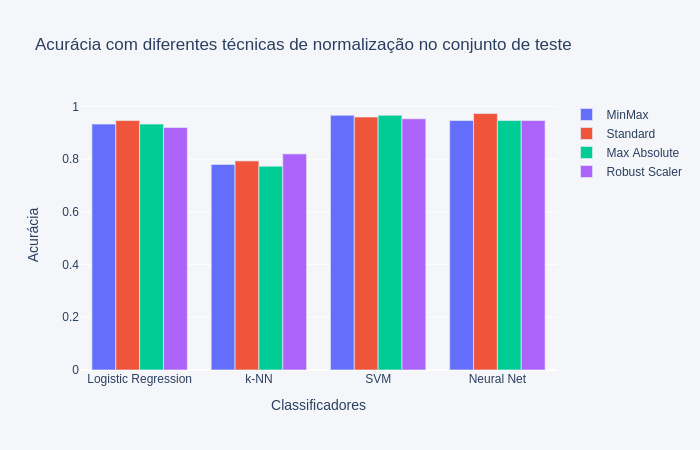
\includegraphics[width=1.0\linewidth,clip=true,trim=0cm 0cm 0cm 0cm, keepaspectratio=true]{bar_norm_all_lbp.png}
	\caption{Comparação de técnicas de normalização com descritor LBP.}
	\label{fig:bar_norm_all_lbp}
\end{figure}

O classificador MLP com a normalização Standard foi a que obteve o melhor resultado, 97\% de acurácia. O pior resultado foi obtido pelo classificador KNN com a normalização Max Absolute, 77\%.

\subsection{Descritor Gabor}
Para o descritor Gabor as diferenças entre os resultados obtidos foi alta para o classificador KNN, contudo nenhum dos classificadores obtiveram 50\% de acurácia. A técnica de normalização Min-Max que consiste em transformar cada característica com valor mínimo em 0 e os valores máximos em 1, sendo que o restando é tranformado em um valor decima entre 0 e 1, obteve a melhor acurácia com o classificador KNN, 41\%. O pior desempenho foi obtido pelo classificador KNN com a normalização Standard, 21\%. Os resultados podem ser vistos na Figura~\ref{fig:bar_norm_all_gabor} Foram mantidos os classificadores utilizados no último experimento.

\begin{figure}[!htbp]
	\centering
	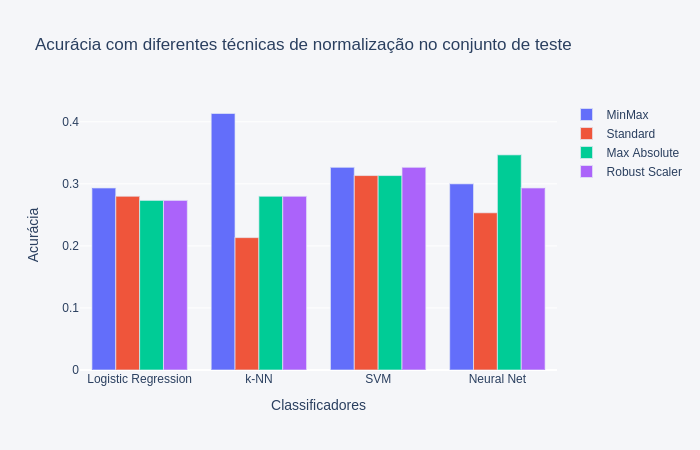
\includegraphics[width=1.0\linewidth,clip=true,trim=0cm 0cm 0cm 0cm, keepaspectratio=true]{bar_norm_all_gabor.png}
	\caption{Comparação de técnicas de normalização com descritor Gabor.}
	\label{fig:bar_norm_all_gabor}
\end{figure}